\documentclass[11pt]{article}

\usepackage{setspace}
\usepackage{inputenc}
\usepackage[margin=1in]{geometry}
\usepackage{subfig}
\usepackage{graphicx}


\title{%
Model Comparison for Bird Species Identification\\
  \large ISyE 6740 - Spring 2022 Project Report}
\author{Team Members: Joe Laniado (GTID: 903233267)}


\begin{document}
\begin{singlespace}
\begin{titlepage}
\maketitle
\end{titlepage}
\tableofcontents
\clearpage

\section{Problem Statement}
Ever since computers were created, we have been trying to find ways for them to automate difficult tasks and make our lives easier. Things like finding the shortest path between two places, drawing a three dimensional floor plan for a new skyscraper, or even doing complex mathematical calculations in seconds; have become as trivial as just opening your phone or laptop and asking a question. One of such questions that came up during the late 1960s was: If we give eyes to a computer, would it know what it was looking at? 
Of course the answer was no, but then the goal became to find a way to teach it how to do it. This was the birth of the scientific field of computer vision. This discipline deals with analyzing, processing, and uderstanding visual data in a way which allows a computer to see an image or video, and be able to extract information and make conclusions from it. Using X-ray scans for automatic diagnosis of lung diseases in patients, or collecting quantitive information about the traffic flow of a city using only a camera; are some notable applications of this that are currently in use. \\

After pondering the applications of such computational advancements while doing some bird watching near my home I started to wonder if there could be a way to use computer vision to simplify the process of identifying our feathered friends. I wanted to develop an image classification model that by training it using labeled pictures of different types of birds; if given new input, it could correctly identify which species the new birds belonged to in a quick and efficient way. This process would save me so much time of manual classification of hundreds of pictures of birds in my camera that I just haven't had the time to sit down and check. Fellow local scientists and bird watching enthusiasts have also expressed excitement over the creation of such a model. Furthermore, out in the field spotting a bird could last only a couple of seconds before it flies away, so any time saved on identifiying the species could be used on monitoring other behaviours or collecting scientific information about such a sight. For this a real time video classifier could be used in order to detect and classify the bird before it flies away, although such a project would be a little more advanced than a simple image classifier. \\

Using the different algorithms learned in class, there is a number of ways to approach the development of our bird species identifier. By means of dimensionality reduction, density estimation, traditional classification algorithms, and deep learning; we will build and compare different image classification models until we find the most accurate and efficient approach to correctly identify the species of each bird. We will evaluate each model with a number of performance variables and analyze their behaviour for this specific classification task. Finally, the best model will be selected and further scalability and functionality implementations will be discussed. 

\section{Data Source}

The original dataset consists of pictures from more than 400 different species of birds. This includes 58388 training images, 2000 test images, and 2000 validation images. When it comes to the images themselves; each picture is a 224 x 224 x 3 RGB image in jpg format, and contains only one bird per image. The bird usually takes more than 50\% of the pixels in the image making it convenient for training purposes. All images were collected from the BIRDS 400 dataset found at https://www.kaggle.com/gpiosenka/100-bird-species. One important thing to note is that 85\% of the images are from the male of the species and only 15\% are female, this is due to the male having more colors and features that make them more easily recognizible. Due to the big size of the data 15 different species were selected in order to save time and reduce complexity when implementing each approach for our classifier. More species could be added whenever an optimal classifier is selected. Figure 1 shows the selected species of birds:\\

\begin{figure}[h]
    \centering
    
    \subfloat[Black Broadbill]{
        \label{ref_lael1}
        \includegraphics[width=0.2\textwidth]{data/birds/train/1BLACK YELLOW BROADBILL/001.JPG}
    }
    \subfloat[Flamingo]{
        \label{ref_lbel4}
        \includegraphics[width=0.2\textwidth]{data/birds/train/2FLAMINGO/011.JPG}
    } 
    \subfloat[Bald Eagle]{
        \label{ref_label1}
        \includegraphics[width=0.2\textwidth]{data/birds/train/3BALD EAGLE/019.JPG}
    }
    \subfloat[Annas Hummingbird]{
        \label{ref_label2}
        \includegraphics[width=0.2\textwidth]{data/birds/train/4ANNAS HUMMINGBIRD/006.JPG}
    }
    \subfloat[Scarlet Macaw]{
        \label{ref_label3}
        \includegraphics[width=0.2\textwidth]{data/birds/train/5SCARLET MACAW/016.JPG}
    }\\
    \subfloat[Abbots Babbler]{
        \label{reflabel1}
        \includegraphics[width=0.2\textwidth]{data/birds/train/7ABBOTTS BABBLER/013.JPG}
    }
    \subfloat[Abbots Booby]{
        \label{ref_lbel2}
        \includegraphics[width=0.2\textwidth]{data/birds/train/8ABBOTTS BOOBY/002.JPG}
    }
    \subfloat[Ground Hornbill]{
        \label{ref_label3}
        \includegraphics[width=0.2\textwidth]{data/birds/train/9ABYSSINIAN GROUND HORNBILL/007.JPG}
    }
    \subfloat[Crowned Crane]{
        \label{rf_label3}
        \includegraphics[width=0.2\textwidth]{data/birds/train/AAFRICAN CROWNED CRANE/018.JPG}
    } 
    \subfloat[Emerald Cuckoo]{
        \label{ef_label4}
        \includegraphics[width=0.2\textwidth]{data/birds/train/AAFRICAN EMERALD CUCKOO/007.JPG}
    }\\
    \subfloat[African Firefinch]{
        \label{ref_lael2}
        \includegraphics[width=0.2\textwidth]{data/birds/train/AAFRICAN FIREFINCH/006.JPG}
    }
    \subfloat[Oyster Catcher]{
        \label{ref_label3}
        \includegraphics[width=0.2\textwidth]{data/birds/train/AAFRICAN OYSTER CATCHER/009.JPG}
    }
    \subfloat[Alberts Towhee]{
        \label{ref_labl3}
        \includegraphics[width=0.2\textwidth]{data/birds/train/AALBERTS TOWHEE/021.JPG}
    }
    \subfloat[Alexandrine Parakeet]{
        \label{ref_labl4}
        \includegraphics[width=0.2\textwidth]{data/birds/train/AALEXANDRINE PARAKEET/017.JPG}
    }
     \subfloat[Touchan]{
        \label{ref_label4}
        \includegraphics[width=0.2\textwidth]{data/birds/train/6TOUCHAN/013.JPG}
    }
    
    
    \caption{Selected Species}
    \label{selected species}
\end{figure}

The following distribution of pictures applies for each species selected:
\begin{itemize}
\item Training: 120
\item Validation: 5
\item Testing: 5
\end{itemize}

The total distribution ends up being 1800 for training, 75 for validation, and 75 for testing. 

\section{Methodology}
\subsection{Data Pre-Processing}

For efficiency purposes each image was resized to be 64x64x3 pixels, they were then vectorized into the form 1x12,288 and collected into three different matrices. One for training, validation, and testing; where each row represented a singular picture, and each column the pixel values. Each matrix was labeled depending on the species it came from and assembled into dictionaries, where the key-value pair was the species name and the specific matrix respectively. It is important to note that the images were not transformed into grayscale due to color being such an important feature when classifying birds. Furthermore, the disparity between male and female specimens was determined that while it would probably introduce some level of error into our model, in this case it would be used to test the generalization to different cases when performing the classification. At least until more data is available.\\

One area of concern was that due to the high variability between picture design, 120 images per species might not be good enough to capture the complexity of poses and states that the bird could present. This would cause our model to overfit and not generalize well when testing new kinds of pictures. To solve this problem, slight data augmention was implemented to increase the number of samples we had. In order to maintain model efficiency while testing different approches, only rotation and flipping were implemented in order to multiply or training images from 1800 to 7200. Operations like cropping, contrast, translation, and more could be used if more training data is needed for future applications. 

\subsection{Dimensionality Reduction}
The first approach implements a dimensionality reduction technique to find the most representative combination of features for each species and then compare it to a test sample to make a classification. We start by defining our training images as a $M$x$N$ matrix X, where $M$ represents the number of samples and $N$ the number of pixels. To better understand the math behind this technique, it is important to know the following concepts:

\begin{enumerate}
\item The theorem for singular value decomposition states that: $ A_{MxN} = U_{NxN}S_{MxN}V_{NxN}$. Where U and V are orthonormal, $U$ represents the left singular vectors, $S$ the singular values, and $V^T$ the right singular vectors.
\item We also know that for a NxN matrix W, there exists an eigenvector u if:
$$ Wu = \lambda u $$ 
Where $\lambda$ is a scalar that represents the eigenvector of $W$. 
\end{enumerate}

The basic Idea of this approach is that for each species of bird, we will find the $K$ principal components that encompasses it's most representative features by means of singular value decomposition. Using this ``Eigenbirds'' we will then find the projection residual between each test image and all the $K$ principal components for each species. The test image will be labeled as the type of bird that produces the lowest residual in this equation. 

\begin{enumerate}
\item We find the mean image $\mu$ for $X$ and use it to center all of our training images. This will help us calculate the covariance matrix C. We will also divide all the data by 255 to scale for computational efficiency. The following operation can be shown as:
$$ \mu = \frac{1}{m}\sum_{i=0}^{m}X_i $$
$$ X = (X-\mu)/255 $$

If we reshape the mean to it's original dimensions and plot it as an image for each species we get the following:

\begin{figure}[h]
    \centering
    
    \subfloat[Black Broadbill]{
        \label{ref_labe1}
        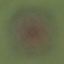
\includegraphics[width=0.2\textwidth]{plots/meanbird-BLA.jpg}
    }
    \subfloat[Flamingo]{
        \label{ref_labe4}
        
\includegraphics[width=0.2\textwidth]{plots/meanbird-FLA.jpg}
    } 
    \subfloat[Bald Eagle]{
        \label{ref_labe1}
        
\includegraphics[width=0.2\textwidth]{plots/meanbird-BAL.jpg}
    }
    \subfloat[Annas Hummingbird]{
        \label{ref_labe2}
        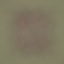
\includegraphics[width=0.2\textwidth]{plots/meanbird-ANN.jpg}
    }
    \subfloat[Scarlet Macaw]{
        \label{ref_labe3}
        
\includegraphics[width=0.2\textwidth]{plots/meanbird-SCA.jpg}
    }
    
    \caption{1st principal component for each species visualized as a picture.}
\end{figure}

\item We can now define our covariance matrix as $ C = XX^T $ which is a symmetrical matrix that can be diagonilized in the form: 
$$ C = ULU^T$$ 
Where U is a matrix of eigenvectors and L is a diagonal matrix with eigenvalues $\lambda_i$- Another approach to calculate the eigenvalues and eigenvectors is to perform SVD on the transpose of our initial matrix X. Furthermore, if we plug our result into C we obtain the relationship between the two methods in calculating our eigenvectors and eigenvalues:
$$ X^T = USV^T  \rightarrow C = USV^TVSU^T = US^2U^T$$
In this case U would represent our principal components and $S^2$ our eigenvalues. If we were to grab the first principal component for the 5 species and visualize it, we would get the following result: \\

\begin{figure}[h]
    \centering
    
    \subfloat[Black Broadbill]{
        \label{ref_labe1}
        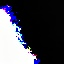
\includegraphics[width=0.2\textwidth]{plots/eigenbird-BLA.jpg}
    }
    \subfloat[Flamingo]{
        \label{ref_labe4}
        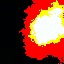
\includegraphics[width=0.2\textwidth]{plots/eigenbird-FLA.jpg}
    } 
    \subfloat[Bald Eagle]{
        \label{ref_labe1}
        
\includegraphics[width=0.2\textwidth]{plots/eigenbird-BAL.jpg}
    }
    \subfloat[Annas Hummingbird]{
        \label{ref_labe2}
        
\includegraphics[width=0.2\textwidth]{plots/eigenbird-ANN.jpg}
    }
    \subfloat[Scarlet Macaw]{
        \label{ref_labe3}
        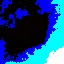
\includegraphics[width=0.2\textwidth]{plots/eigenbird-SCA.jpg}
    }
    
    \caption{1st principal component for each species visualized as a picture.}
\end{figure}

Due to each principal component representing a very small amount of variance only very fine details and combinations of color values con be seen in each image. it may appear random but when put together with the rest of principal components we get a pretty good estimate of the most significant features for each species.\\


\item Finally, for each test image $y_i$ and each species $j$; we find the projection residual by:

$$ Z_i = (y_i - \mu_j )/255$$
$$ Projection Residual = || Z_i - U_jU_j^TZ_i ||^2_2 $$

Where $Z_i$ is the centered vector for image $y_i$ using the mean $\mu_j$ of species $j$. After looping through each test image - species combination, the result will be a MxK matrix where each row represents one of $M$ test images and each column the residual when compared to all $K$ species. All is left to do is to find the minimum residual in each row, and that will give us the predicted species for each image. 
\end{enumerate}

The question remains of choosing how many principal components to use when calculating our projection residual. This can be addresed by plotting the variance percentage for each principal component and selecting the ones that explain most of the variance in the data. In this case, after performing SVD for the first 5 species of birds and getting the respective eigenvalues, each one was scaled between 1 and 0 and converted into percentages. They were then plotted in figure 2 to show the explained variance of each principal components for each species. \\

\begin{figure}[h]
    \centering
    
    \subfloat[Black Broadbill]{
        \label{ref_labe1}
        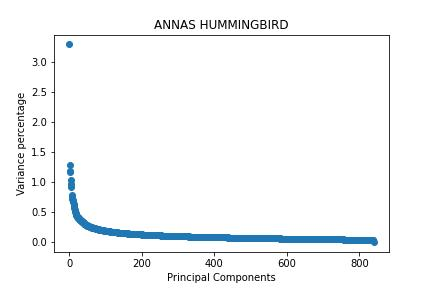
\includegraphics[width=0.33\textwidth]{plots/variance-ANN.jpg}
    }
    \subfloat[Flamingo]{
        \label{ref_labe4}
        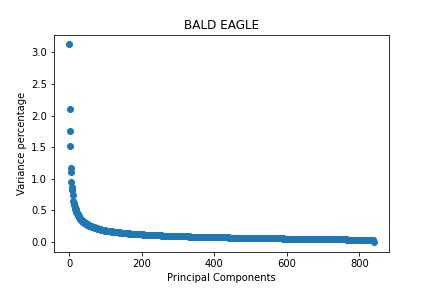
\includegraphics[width=0.33\textwidth]{plots/variance-BAL.jpg}
    } 
    \subfloat[Bald Eagle]{
        \label{ref_labe1}
        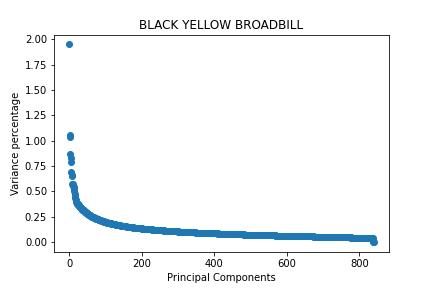
\includegraphics[width=0.33\textwidth]{plots/variance-BLA.jpg}
    }\\
    \subfloat[Annas Hummingbird]{
        \label{ref_labe2}
        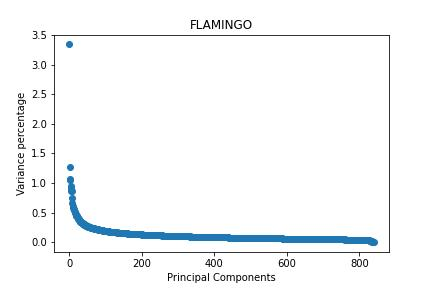
\includegraphics[width=0.33\textwidth]{plots/variance-FLA.jpg}
    }
    \subfloat[Scarlet Macaw]{
        \label{ref_labe3}
        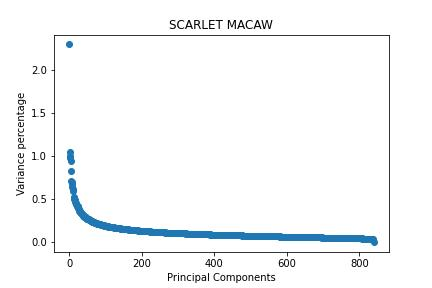
\includegraphics[width=0.33\textwidth]{plots/variance-SCA.jpg}
    }
    
    \caption{Selected Species}
\end{figure}

We can see how most of the plots have a similar distribution of variance for each principal component and how around the 100 level mark seems to level off. It was decided that using the first 90 principal components would encompess the most menaingful features of each bird, and would be the parameter used in our model. Therefore, using the first 90 principal components we calculated the residuals for each one of our test images against each species, then by choosing the lowest residual the image was classified respectively. The time it took for the model to run from image input to image classification was taking into account as a measure of model efficiency. It took 3475.41 seconds to complete or around 57.92 minutes. The following were the results: \\
\begin{figure}[h]
    \centering
    
    \subfloat[Classification Metrics]{
        \label{ref_labe1}
        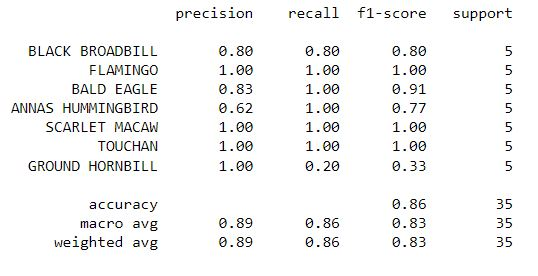
\includegraphics[width=0.5\textwidth]{plots/dim-red-results.jpg}
    }
    \subfloat[Confusion Matrix]{
        \label{ref_labe4}
        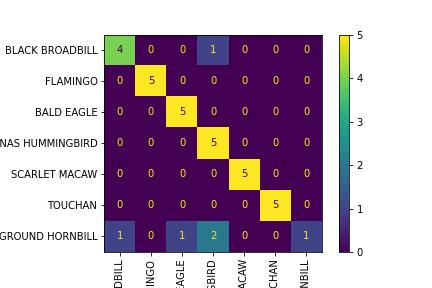
\includegraphics[width=0.6\textwidth]{plots/dim-red-cf.jpg}
    }
    \caption{Dimensionality Reduction Evaluation.}
\end{figure} 


\subsection{Density Estimation}

Density estimation is another method that can be used to build a species identifier. This method is an unsupervised learning technique that is used to find where similar data clusters together due to having similar features. Clustering is a technique that takes advantage of density estimation through different dimensions for multivariate data. In this case, a non-parametric approach called Kmeans clustering will be used on our training images to find which images are the most similar to each other, in effect creating $D$ clusters that based on certain features each one is classified as a type of bird. Using a new test image $y$, then we can use our model to predict to which cluster y is more similar to. Once assigned to a cluster we calculate the majority label of the cluster given all the data points assigned to it. This will be our new label for image $y$. \\

More specifically, the pre-processed data was used to build our training matrix $A$ where each row represents an image vector, and each column represents the pixel values of said vector. The entire matrix was then scaled by 255 to bound our data between 0 and 1, this was due to simplify computational load when computing the algorithm. The training images were then passed into our Kmeans algorithm which calulates $K$ clusters centroids randomly, and assigns the closes data points to each centroid. Each data point is then labeled based on which centroid is closest to it. The centroids are then recalculated as the average of all the center of all the data points, and the process then repeats iteratively until no there is no change. The dimensions for each data point will be the pixel values for each one of the pictures. The number of clusters will be selected by calculating the model accuracy using a validation set of images in the same matrix format as our training data. Using a range between 15 and 150 clusters in 10 point increments we got the following result on the validation data: \\

\begin{figure}[h]
    \centering
    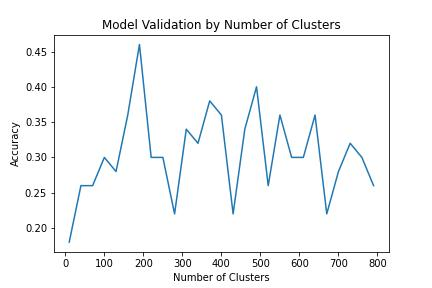
\includegraphics[width=0.5\textwidth]{plots/den-est-valid.jpg}
    \caption{Accuracy Score by number of clusters using Kmeans.}
\end{figure}

Using the results in the validation data we can choose the number of clusters that gave the highest score and build our clustering model. For new test images all we have to do is predict to which cluster it would belong to and assign the majority label of that cluster. It is important to note that the number of clusters doesn't need to match the number of species as each cluster can encompass different aspects of the same species. The time it took for the model to run from image input to image classification was taking into account as a measure of model efficiency. It took seconds to complete or around 57.92 minutes and the following were the results: \\

\begin{figure}[h]
    \centering
    
    \subfloat[Classification Metrics]{
        \label{ref_labe1}
        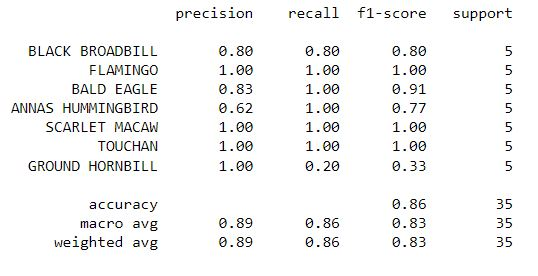
\includegraphics[width=0.5\textwidth]{plots/dim-red-results.jpg}
    }
    \subfloat[Confusion Matrix]{
        \label{ref_labe4}
        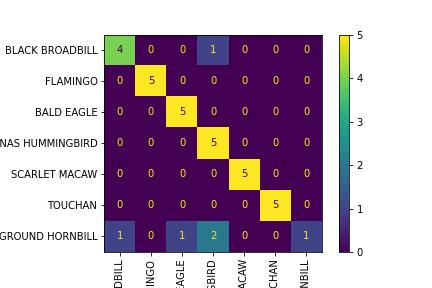
\includegraphics[width=0.6\textwidth]{plots/dim-red-cf.jpg}
    }
    \caption{Dimensionality Reduction Evaluation.}
\end{figure} 


\subsection{Classification}
It is intuitive that some of the first approaches when making a classification of labeled data, are the classic supervised learning models that are so popular when using tabular data. Algorithms like SVM, Kernel SVM, K-nearest neighbors, Naive Bayes, Logistic Regression, and many others. In this section some of those algorithms will be implemented and evaluated to find the best traditional approach for creating our bird classifier. \\



 We will compare them all and discuss the disadvantages and advantages of using each. Classification and model specific metrics will be presented for technique evaluation, and seeing which one is more efficient for the task. Some of this algorithms might be computationally expensive to use due to the big number of data, if this is the case the results will be presented as such and given as a suboptimal solution to our problem. More experiments will be done regarding this case. 

\subsection{Deep Learning}
Our final approach consists of diving into the field of deep learning for image classification. Deep learning is a subfield of machine learning that specializes on reproducing the way the human brain thinks to solve certain problems. It does this by using artificial neural networks; a mathematical representation of a composition of neurons signaling to each other. This field has proven to have an endless number of real life applications when it comes to using data to gain insight on an input. In this case, we will implement a variation of this approach called a convolutional neural network. This algorithm is specifically designed to deal with the high dimensionality that images present. It is important to note that for an 64x64x3 image the number of dimensions that each alogrithm has to take into account is 12,288, combined with more than 7000 distinct training images we get more than 80,000,000 distinct values that need to be taken into account. Performing the neccesary computations to learn from the data becomes a tedious and long task to do in a normal computer. CNNs solve this issue by taking advantage of two ideas: Convolutions and subsampling. Convolution is the process of extracting the high level features of an image through the use of a filter, for each feature we perform subsampling to reduce the spatial size of the convolved feature to reduce the computational power necessary for the algorithm to work. We alternate between this two methods in the form of layers until we come out with an output that has been trained to understand the features of each species. this output will be flattened into a vector and fed into a traditional feed forward neural network to make our classification. Due to this small amount of training images we might have a tendency to overfit to our training data and fail to generalize properly when validating our model. To prevent this, some neurons will be turn off randomly during the training process to prevent the network becoming too dependent in the data. This concept is known as dropout as is used as a regularization tool when using CNNs. \\

For this approach the training data was reshaped into a 4 dimensional matrix of shape Mx64x64x3 to serve as an input to our network. One-hot encoding was performed to each of our training labels as well to transform it into a 1 dimensional vector which combined between all the training images gives us a matrix of size MxK, where each row represents the label vector of each training image and each column the species that it belongs to. For our network, each layer consisted of a convolution step, a leaky relu activation function to capture non-linear relationships, and a max pooling step that serves as our subsampling for that layer. Dropout was implemented aswell after each layer and finally a dense layer was added to input our flatten data and make our classification. The summary of the network can be seen below: \\

\begin{figure}[h]
    \centering
    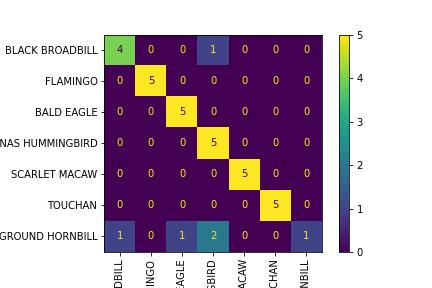
\includegraphics[width=0.6\textwidth]{plots/dim-red-cf.jpg}
    \caption{Dimensionality Reduction Evaluation.}
\end{figure} 

A batch size of 64 was specified and the network was set up to run for 20 epochs. The network was set up to calculate accuracy as well as loss of the network on a validation set at each epoch. This data was saved and plotted for evaluation purposes. The following is the result: \\

\begin{figure}[h]
    \centering
    
    \subfloat[Classification Metrics]{
        \label{ref_labe1}
        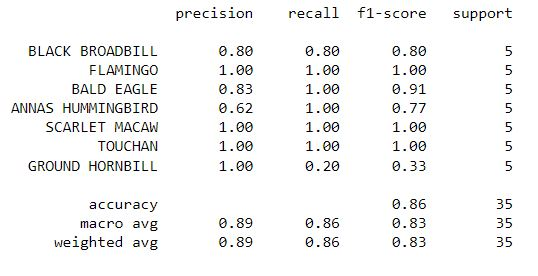
\includegraphics[width=0.5\textwidth]{plots/dim-red-results.jpg}
    }
    \subfloat[Confusion Matrix]{
        \label{ref_labe4}
        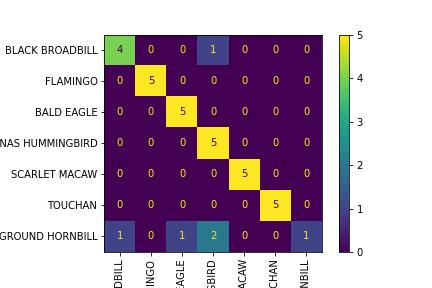
\includegraphics[width=0.6\textwidth]{plots/dim-red-cf.jpg}
    }
    \caption{Dimensionality Reduction Evaluation.}
\end{figure} 

Finally, we evaluate our model on the test data and plot the results: \\

\begin{figure}[h]
    \centering
    
    \subfloat[Classification Metrics]{
        \label{ref_labe1}
        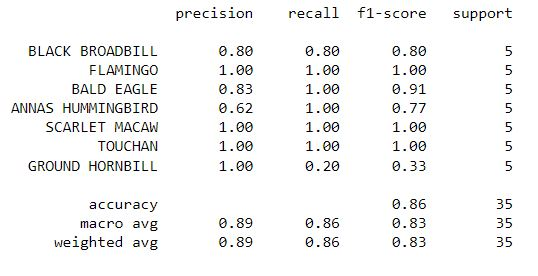
\includegraphics[width=0.5\textwidth]{plots/dim-red-results.jpg}
    }
    \subfloat[Confusion Matrix]{
        \label{ref_labe4}
        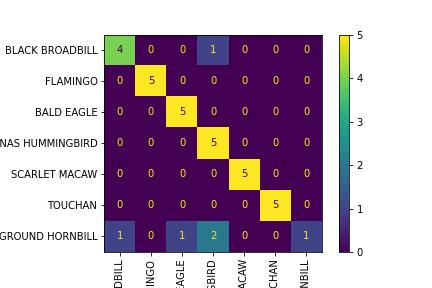
\includegraphics[width=0.6\textwidth]{plots/dim-red-cf.jpg}
    }
    \caption{Dimensionality Reduction Evaluation.}
\end{figure}



\section{Evaluation and Final Results}

In this final section the most meaningful metrics from each one of the 4 applied techniques will be presented and compared. Further discussion on the performance of each and further aplications will be mentioned. Testing with a higher number of data will also be performed at this stage to see how the best technique generalizes when presented with a more real world example. Using our better perfoming approach, we will build our bird species identifier and give the final evaluation metrics of it's implementation. If good results are obtained from initial experiments and no big issues arise while developing each one of the models, a video classifier that takes one frame every $j$ frames and which outputs a label if a bird appears in one of them, might be a good real life implementation of our optimal approach. This will only be done if the scope of this project doesn't prove to be too heavy on one person. If not, scalibility and further possibilities will also be discussed in the conclusion section. 



\end{singlespace}
\end{document}
